\chapter{Benutzerschnittstelle der Semanitc-Lifiting-Engine}
\label{benutzer}

Die Semantic-Lifting Funktionalitäten können in Eclipse über ein dafür angelegtes \textit{Action
Set} ausgewählt werden (Abbildung \ref{fig:semantic_lifting_dialog} (links)). Durch ein \textit{Action
Set} lässt sich die Eclipse Plattform um Menüs und Werkzeugleisten-Einträge erweitern. 

\begin{figure}[htb]
  \centering
  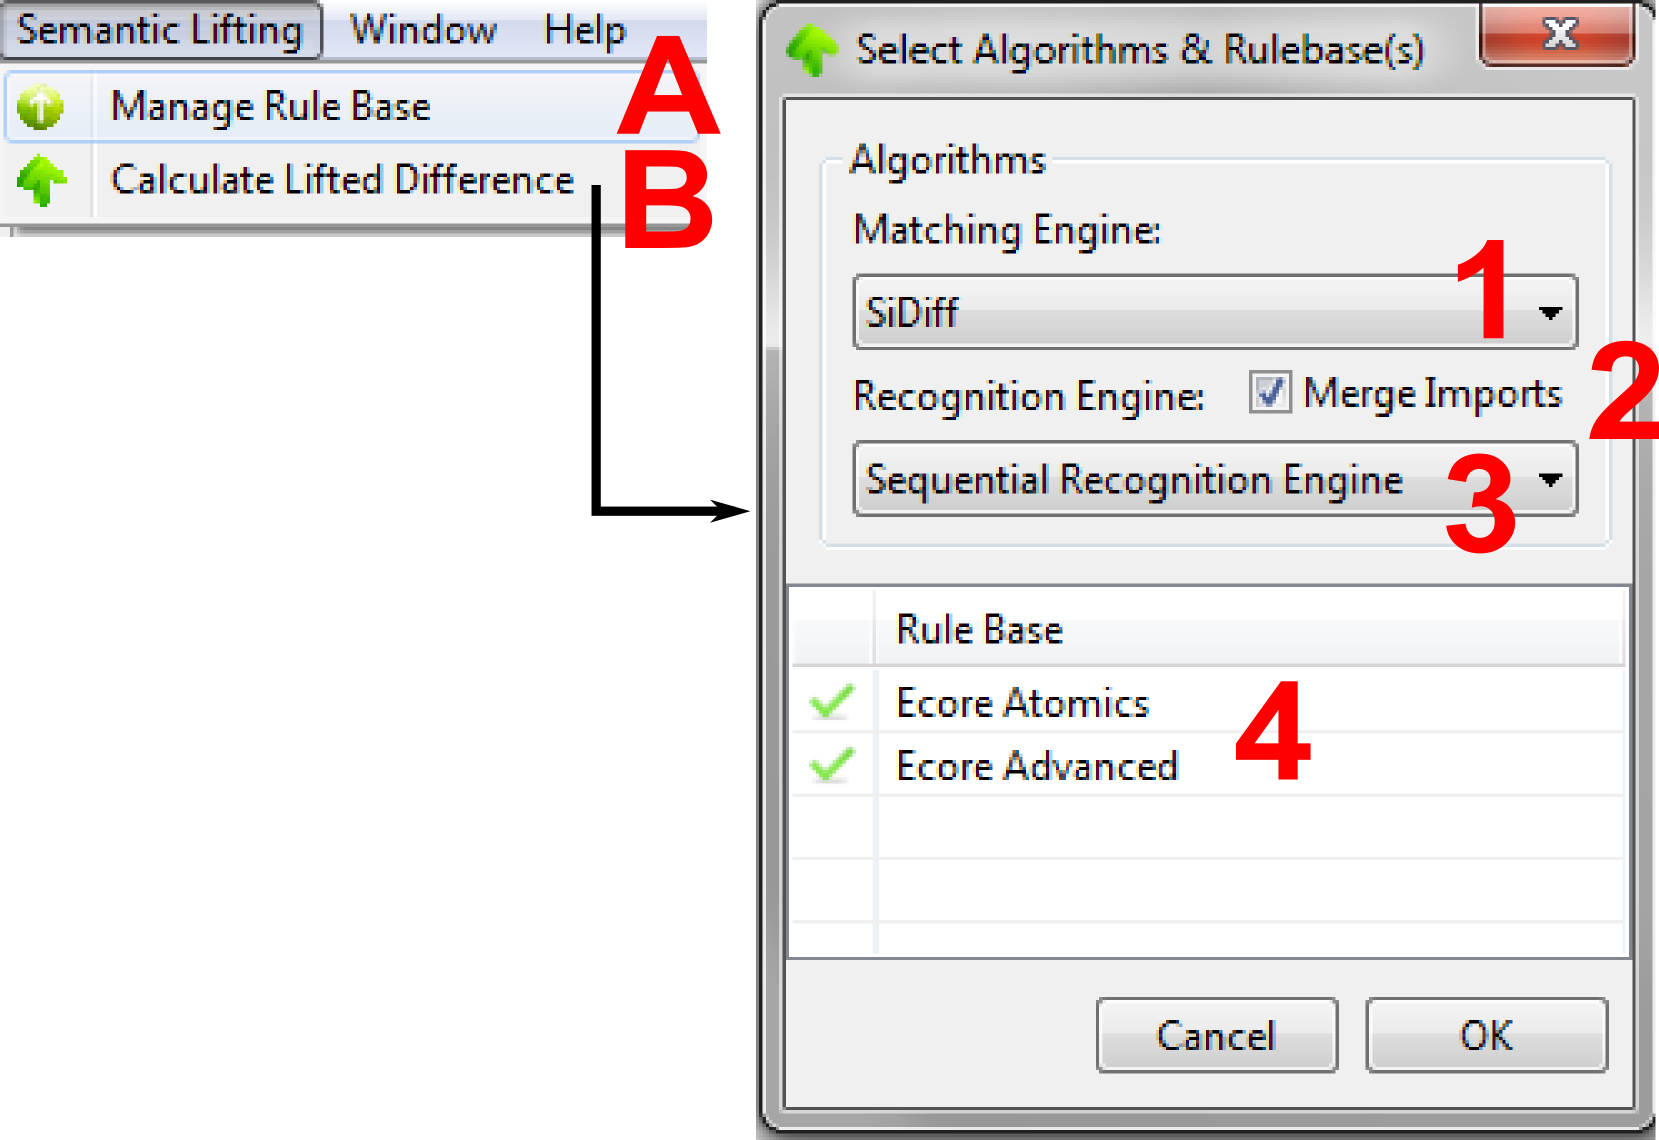
\includegraphics[scale=0.8]{images/semantic_lifting_dialog.png}
  \caption{Semantic-Lifting Dialog}
  \label{fig:semantic_lifting_dialog}
\end{figure}

\begin{itemize}
  \item[\textbf{A:}] Startet die in Abschnitt \ref{verwaltung} beschriebene Regelbasis-Verwaltung.
 
  \item[\textbf{B:}] Startet einen Dialog, mit dem die Semantic-Lifting-Engine gesteuert werden
  kann. Zunächst muss der Benutzer entscheiden, ob er eine neue technische Differenz berechnen will
  oder ob eine bereits bestehende technische Differenz geladen und geliftet werden soll. Als nächstes wird dann
  ein Dateidialog gestartet, in dem entsprechend der zuvor getroffenen Auswahl entweder eine
  ungeliftete technische Differenz oder zwei zu vergleichende Modelle (Modell A und B) auszuwählen
  sind. Als nächstes wird der in Abbildung \ref{fig:semantic_lifting_dialog} (rechts) gezeigte
  Dialog aufgerufen.

  \item[\textbf{1:}] Hier können die in Abschnitt \ref{sec:matching} beschriebenen
  Vergleichsalgorithmen ausgewählt werden, durch die die Korrespondenzen zwischen Modell A und B
  berechnet werden. Zur Auswahl stehen \textit{SiDiff} (Abschnitt \ref{sidiff}) und der
  \textit{Named-Element-Matcher} (Abschnitt \ref{nem}). Diese Option kann nur gewählt werden, wenn
  zu Beginn zwei neu zu vergleichende Modelle ausgewählt wurden.
  
  \item[\textbf{2:}] Durch die Option \textit{Merge Imports} kann der Algorithmus zur Behandlung
  von importierten Modellen in Resource-Sets an- und abgeschaltet werden (Abschnitt
  \ref{resource_sets}).
 
  \item[\textbf{3:}] An dieser Stelle werden die Algorithmen für das Semantic-Lifting ausgewählt.
  Es stehen folgende Optionen zur Verfügung.
  \begin{itemize}
    \item \textbf{No Semantic Lifting:} Es wird kein Semantic-Lifting durchgeführt. Dadurch wird
    eine ungeliftete technische Differenz erstellt, wenn zu Beginn zwei Modelle zum Vergleich
    ausgewählt wurden.
    
    \item \textbf{Simple Recognition Engine:} Die technische Differenz wird nur semantisch geliftet.
    Es wird allerdings kein Post-Processing durchgeführt, daher können überlappende
    Semantic-Change-Sets in der Differenz auftreten.
    
    \item \textbf{Post Processed Recognition Engine:} Es wird eine semantisch geliftete und durch
    das Post-Processing überschneidungsfreie Differenz berechnet.
    
    \item \textbf{Sequential Recognition Engine:} Es wird eine semantisch geliftete Differenz mit
    dem unter Abschnitt \ref{sequential} beschriebenen Algorithmus berechnet. Hierdurch werden auch
    die Editieroperationen erkannt, die in sequentieller Abhängigkeit zueinander stehen.
  \end{itemize}
 
  \item[\textbf{4:}] Hier werden alle Regelbasen angezeigt, deren Dokumenttyp dem Metamodell von
  Modell A und Modell B entsprechen. Die einzelnen Regelbasen können für das Semantic-Lifting an-
  und abgewählt werden. Die Regelbasen werden, wie in Abschnitt \ref{verwaltung} beschrieben, als
  \textit{Extension Point} über die \textit{Extension Registry} der Eclipse Plattform ausgelesen. 
\end{itemize}
Nach diesem Dialog wird die Differenzberechnung mit den ausgewählten Optionen gestartet. Nachdem die
Differenz gespeichert wurde, kann diese in dem durch Ecore generierten Editor angezeigt werden. Der
Editor wurde so angepasst, dass alle low-level Änderungen, die geliftet wurden, auch als Gruppierung
unterhalb der Semantic-Change-Sets angezeigt werden. Alle nicht gruppierte low-level Änderungen
werden mit der Differenz als Container angezeigt, wie in Abbildung \ref{fig:lifting_sample} zu sehen
ist. Hier wurden zwei Modell Versionen aus dem EMF Projekt (org.eclipse.emf.codegen.ecore)
verglichen, wobei hier keine sequentiell abhängigen Editieroperationen geliftet wurden, daher sind
ein paar low-level Änderungen ungruppiert, die sonst gruppiert wären.

\begin{figure}[htb]
  \centering
  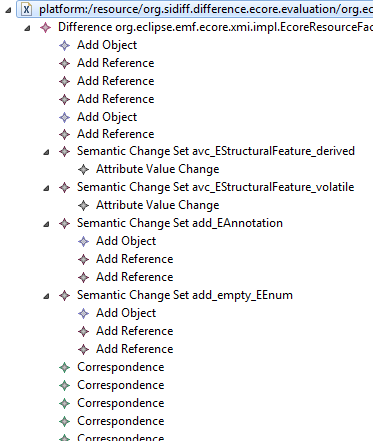
\includegraphics[scale=1.0]{images/lifting_sample.png}
  \caption{Anzeigen der semantisch gelifteten Differenz}
  \label{fig:lifting_sample}
\end{figure}
